\section{External Interface Requirements}
\subsection{User Interfaces}
The following mockups provide a model of graphic interface that will show our program. \\
We will create a user interface that will be user friendly in order to be easy to use also from non-technical users. \\
We list the following mockups that cover all application main aspects: \\

\begin{figure*}
	\begin{minipage}{0.48\textwidth}
		\centering
		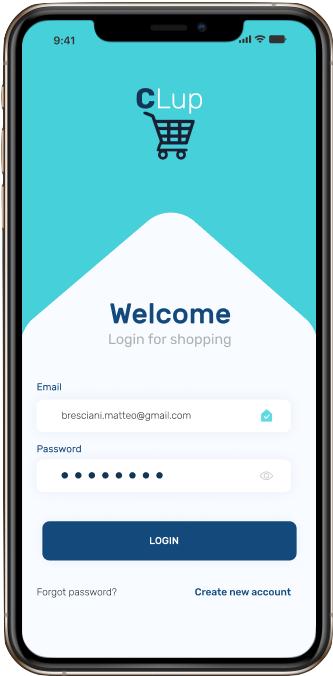
\includegraphics[scale=0.35]{images/login.png}
		\caption{Login}
	\end{minipage}
	\hfill
	\begin{minipage}{0.48\textwidth}
		\centering
		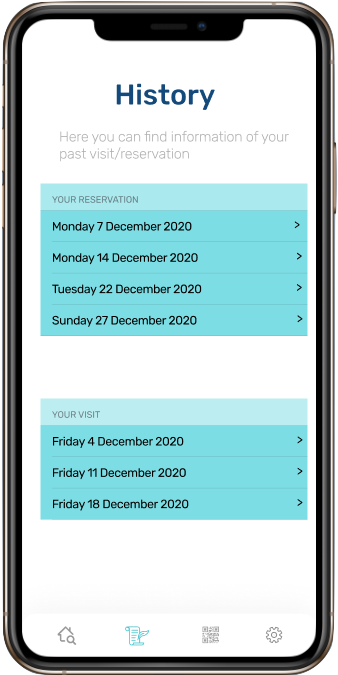
\includegraphics[scale=0.35]{images/history.png}
		\caption{History}
	\end{minipage}
\end{figure*}

\begin{figure*}
	\begin{minipage}{0.48\textwidth}
		\centering
		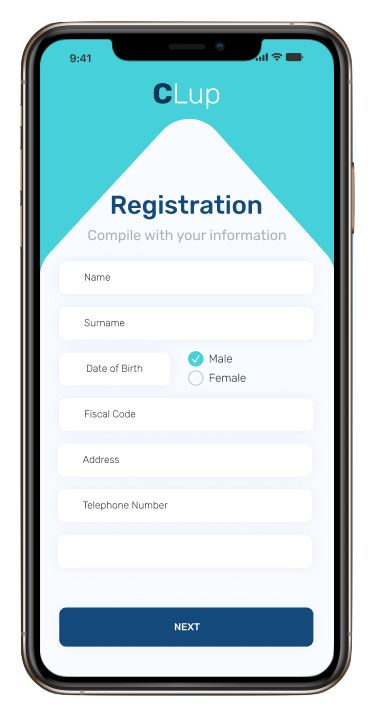
\includegraphics[scale=0.35]{images/reg1.png}
		\caption{Registration 1}
	\end{minipage}
	\hfill
	\begin{minipage}{0.48\textwidth}
		\centering
		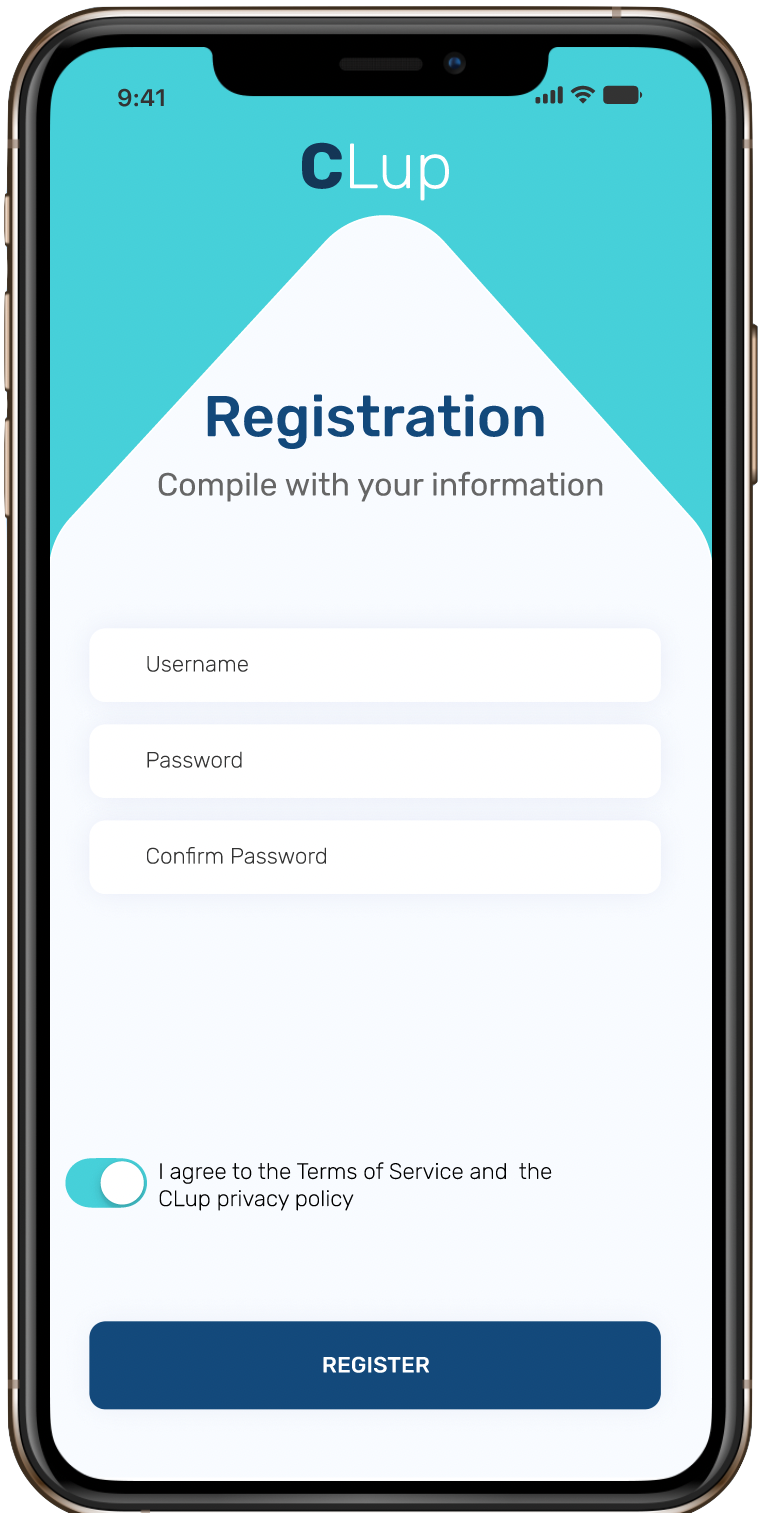
\includegraphics[scale=0.35]{images/reg2.png}
		\caption{Registration 2}
	\end{minipage}
\end{figure*}


\begin{figure*}
	\begin{minipage}{0.48\textwidth}
		\centering
		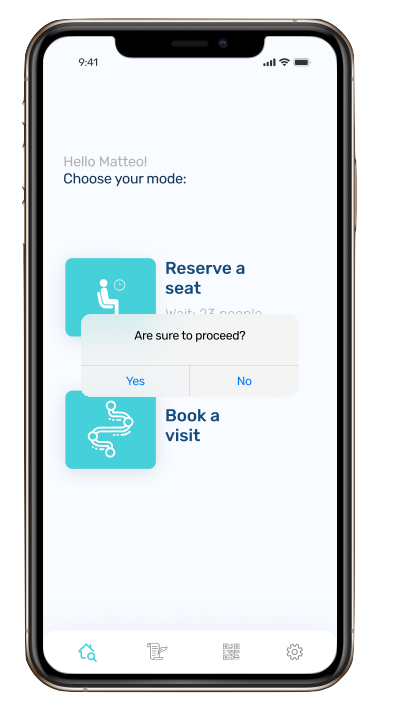
\includegraphics[scale=0.35]{images/reserve1.png}
		\caption{Reservation}
	\end{minipage}
	\hfill
	\begin{minipage}{0.48\textwidth}
		\centering
		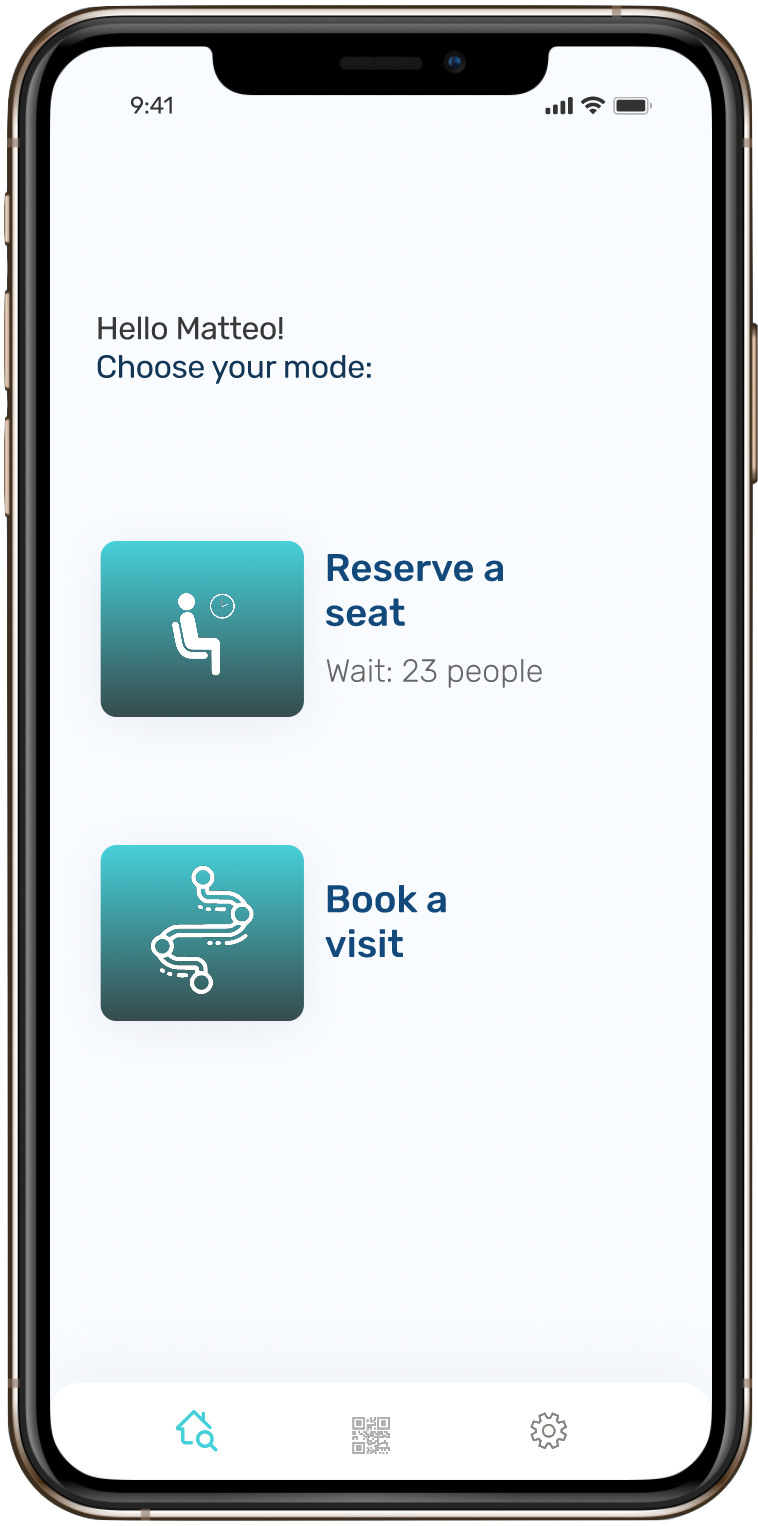
\includegraphics[scale=0.35]{images/home1.png}
		\caption{Home page}
	\end{minipage}
\end{figure*}

\begin{figure*}
	\begin{minipage}{0.48\textwidth}
		\centering
		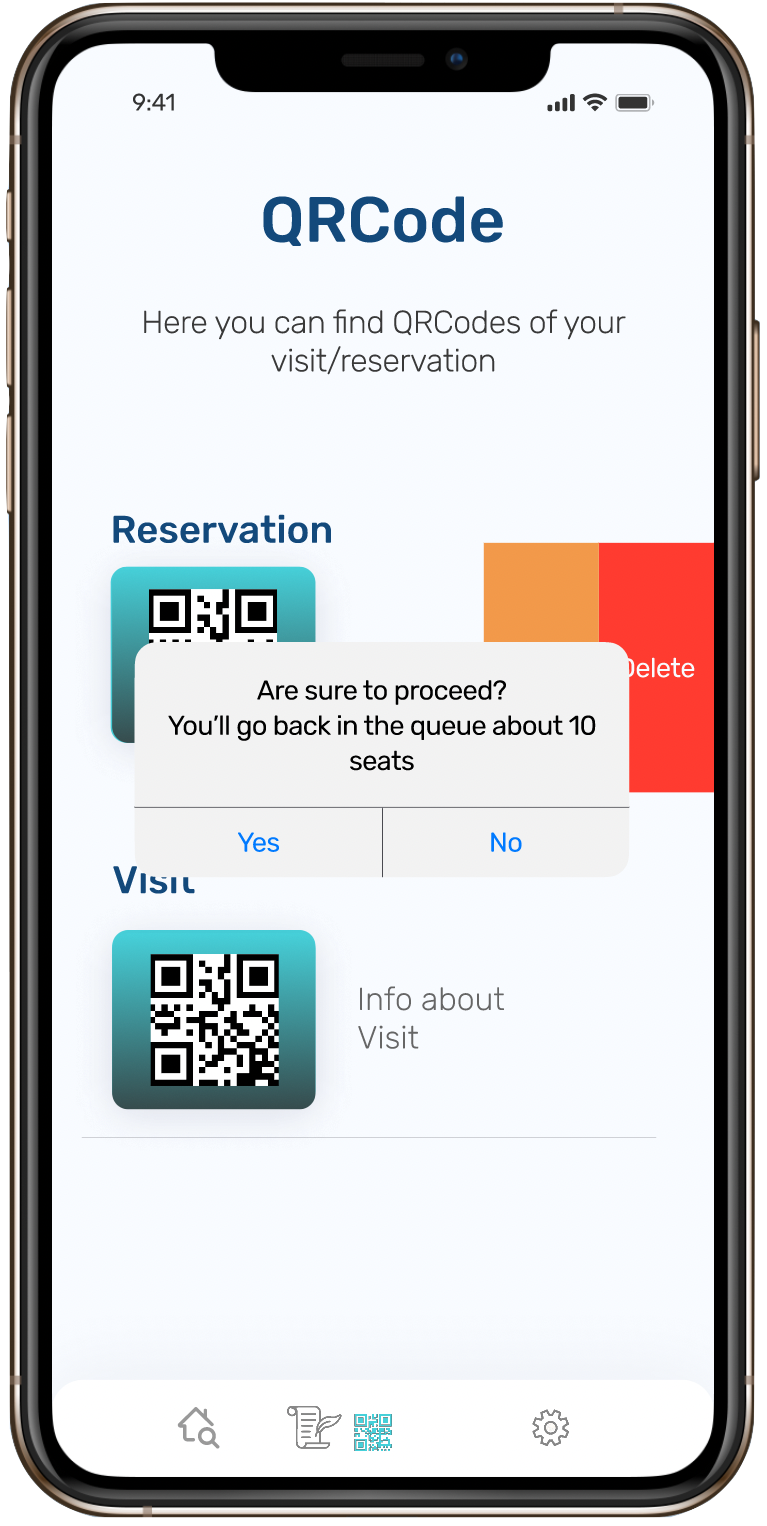
\includegraphics[scale=0.35]{images/qr1.png}
		\caption{Delay}
	\end{minipage}
	\hfill
	\begin{minipage}{0.48\textwidth}
		\centering
		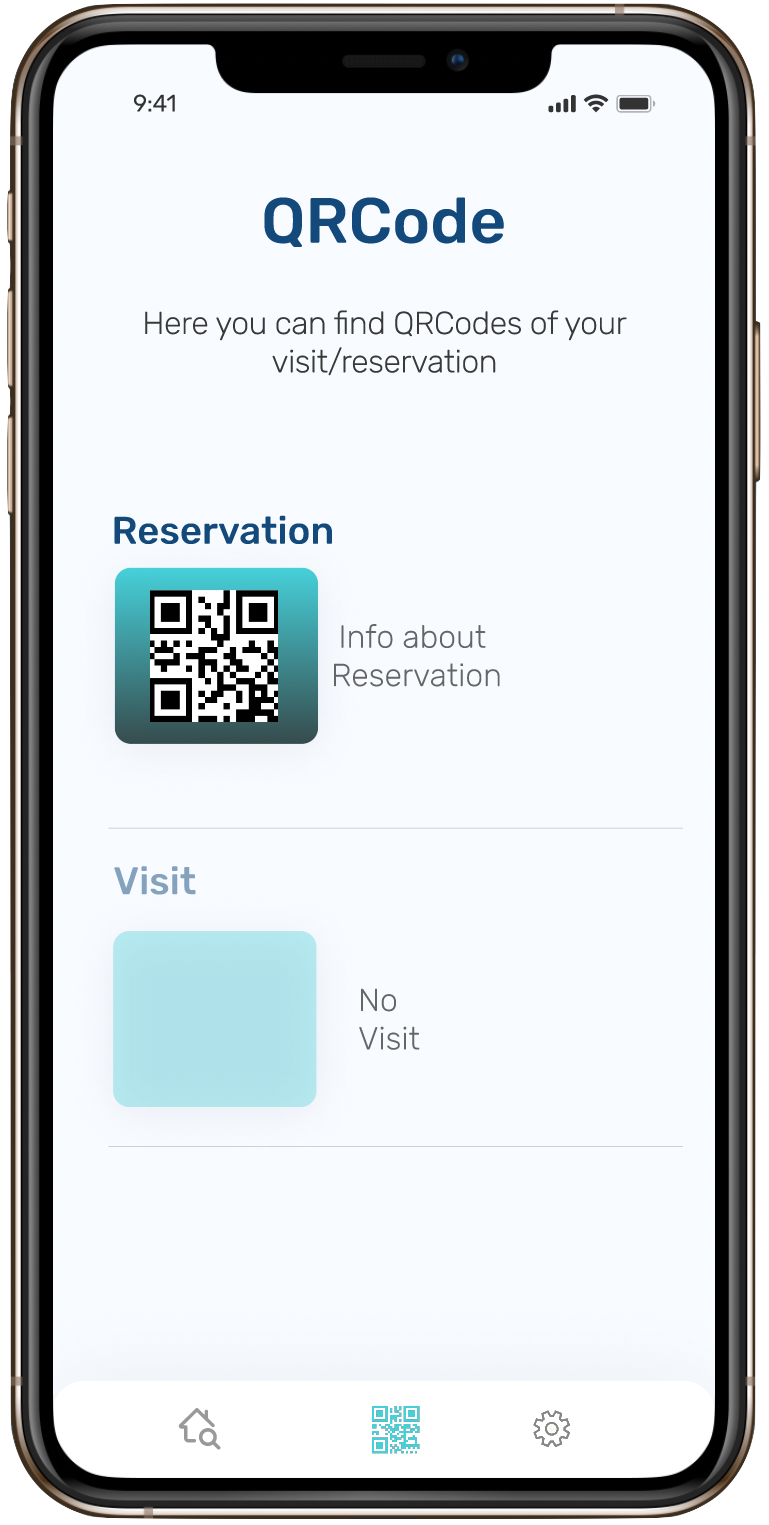
\includegraphics[scale=0.35]{images/qr2.png}
		\caption{Qr code menù 1}
	\end{minipage}
\end{figure*}

\begin{figure*}
	\begin{minipage}{0.48\textwidth}
		\centering
		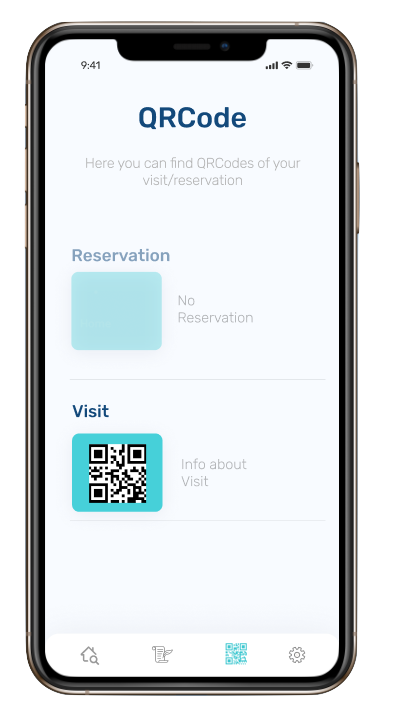
\includegraphics[scale=0.35]{images/qr3.png}
		\caption{Qr code menù 2}
	\end{minipage}
	\hfill
	\begin{minipage}{0.48\textwidth}
		\centering
		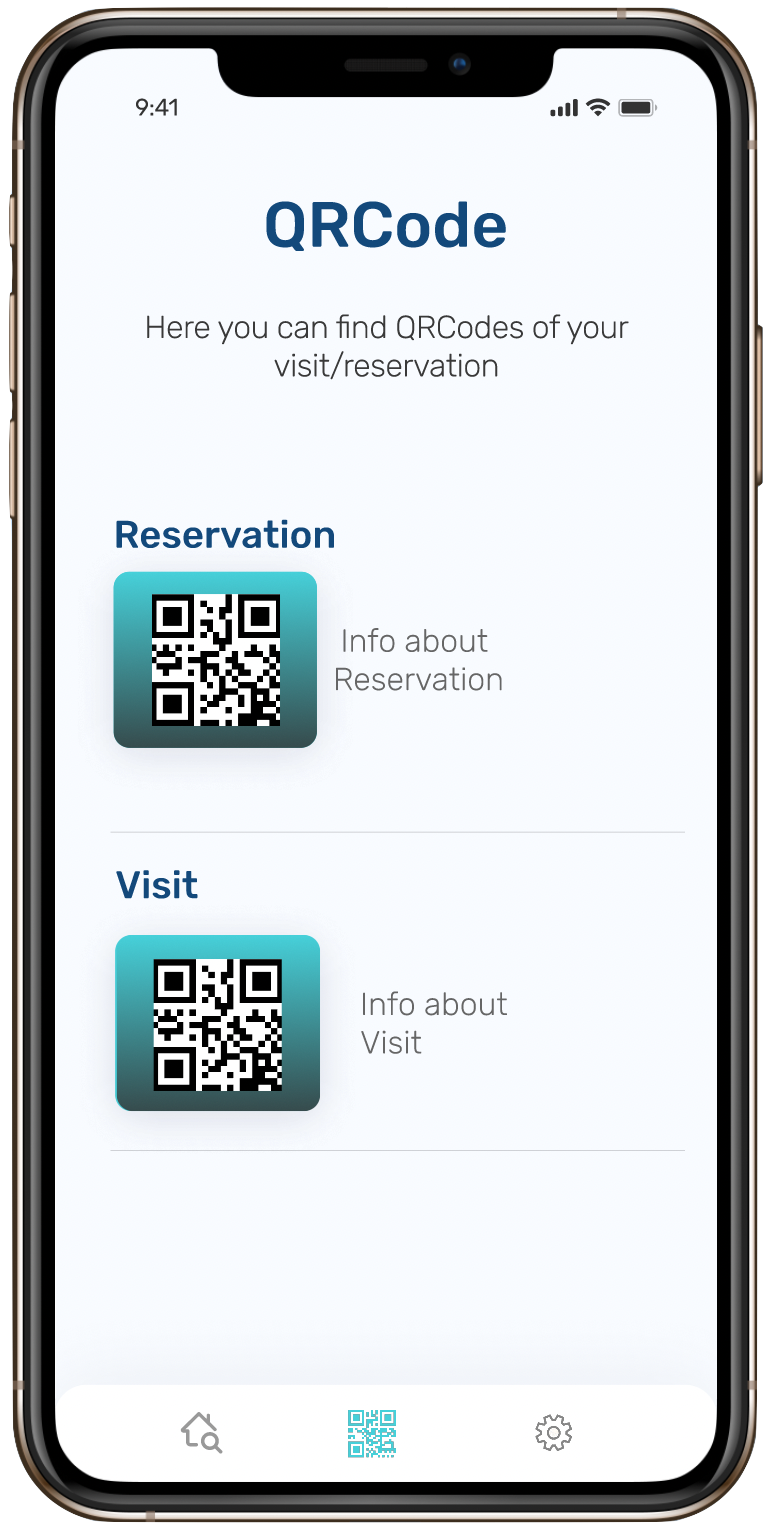
\includegraphics[scale=0.35]{images/qr4.png}
		\caption{Qr code menù 3}
	\end{minipage}
\end{figure*}

\begin{figure*}
	\begin{minipage}{0.48\textwidth}
		\centering
		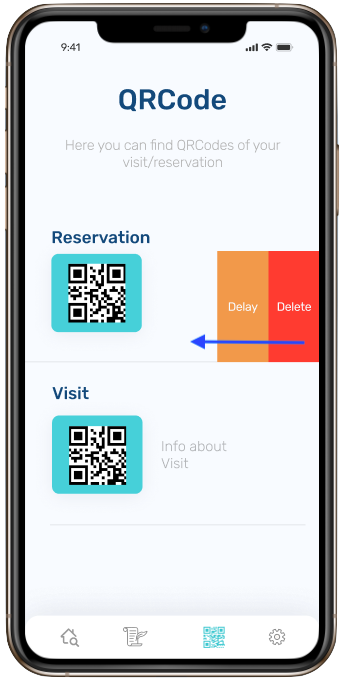
\includegraphics[scale=0.35]{images/qr5.png}
		\caption{Qr code menù 4}
	\end{minipage}
	\hfill
	\begin{minipage}{0.48\textwidth}
		\centering
		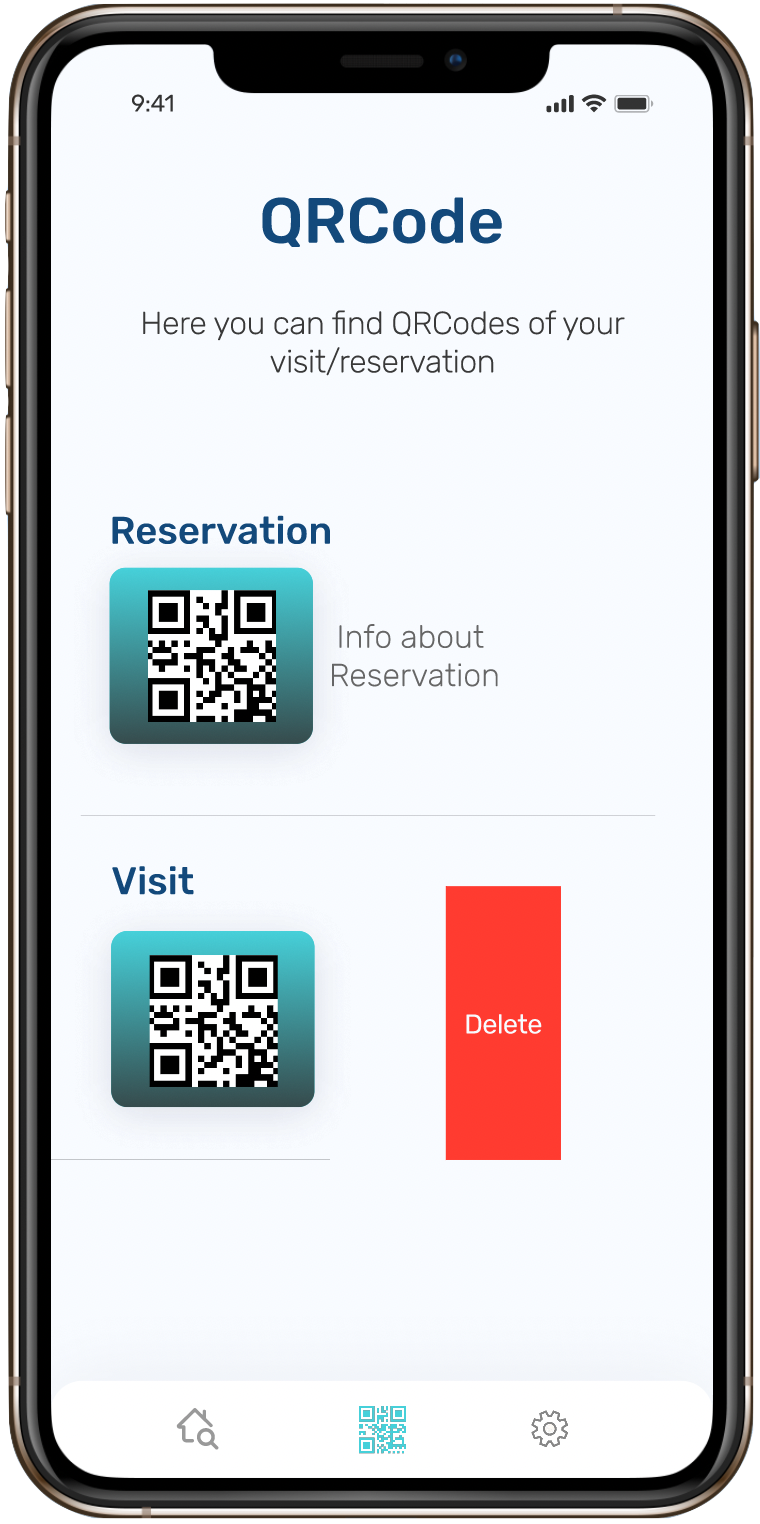
\includegraphics[scale=0.35]{images/qr6.png}
		\caption{Qr code menù 5}
	\end{minipage}
\end{figure*}

\begin{figure*}
	\begin{minipage}{0.48\textwidth}
		\centering
		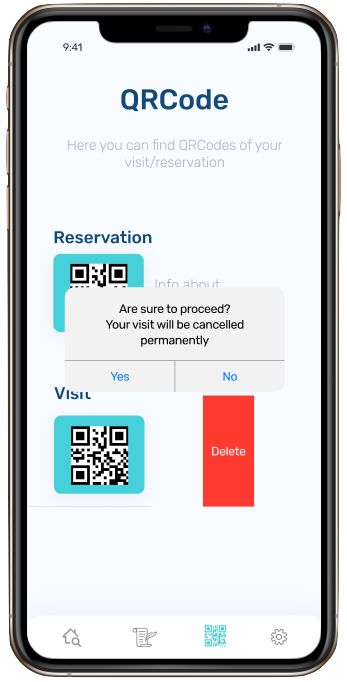
\includegraphics[scale=0.35]{images/qr7.png}
		\caption{Qr code menù 6}
	\end{minipage}
	\hfill
	\begin{minipage}{0.48\textwidth}
		\centering
		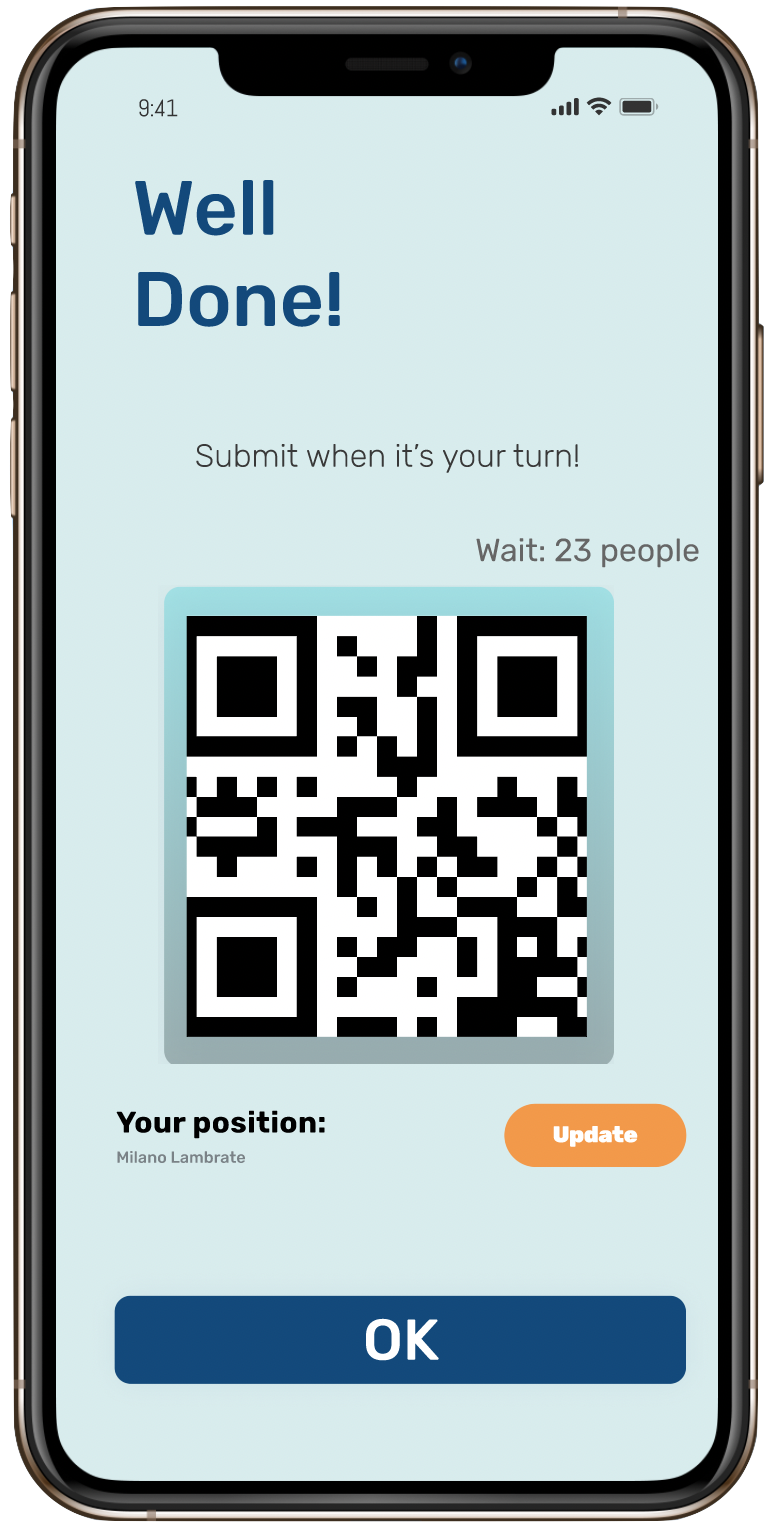
\includegraphics[scale=0.35]{images/qrcode_reservation_done.png}
		\caption{qrcode reservation}
	\end{minipage}
\end{figure*}


\subsection{Hardware Interfaces}


To validate the reservation the supermarket will have two scanners:

\par \medskip 
\begin{itemize}
\item	One at the entry, that will read QR code and will confirm client reservations in case they will be valid. \\
The scanner will reject reservation if QR code will result invalid or will have passed to much time from its call.
\item One at the exit, that when clients will finish shopping allow them to exit to supermarket opening the doors. \\
Another features of exit QR code is to monitor the numbers of client into the shop.
\end{itemize} 
\par \medskip 
The scanners will be used to obtain useful information about client shopping time.

\subsection{Software Interfaces}
\subsection{Communication Interfaces}
\section{Functional Requirements}
\subsection{User}
\par \medskip
{\large \textbf{Scenarios}}
\par \medskip
{\normalsize \textbf{Scenario 1}}
\par \medskip
Giovanna, a career woman who is always in trouble to find free time, needs to go grocery shopping for her family. \\ 
Indeed, once she finished working, she goes to the market and, due to the lockdown, have to wait in line for hours to have access to it. \\
The result is that, coming back home later, she can't put some time in her children.\\
However, in the past days, she discovered CLup App which allows her to book a visit in the market in advance, by only putting the range time avaiable and the size of the expenditure.\\
In this way, Giovanna will save a lot of time and will stay longer with her children, instead of waiting in line outside the market.\\
Nevertheless, due to Covid-19 emergency, the market will be always filled.
\par \medskip 
{\normalsize \textbf{Scenario 2}}
\par \medskip
Jonhathan, an elderly person, on the advice of his grandchild, bought a new smartphone.\\
In addition started using it and installing usefull applications like CLup.\\
In particular, with it, he'll be able to make a reservation in market's queue.\\
In this way, CLup will notify him when, accordingly to his position, leave to get the market in time for his turn.\\
Finally, once he arrived, can go in there by simply scanning the QRCode sent before. \\
At the end Jonhathan will go shopping without waiting on feet his turn during a cold winter's day.\\
\par \medskip 

\begin{figure}[h]
	\caption{Use case USER}
	\label{fig:UML}
	
	\centering
	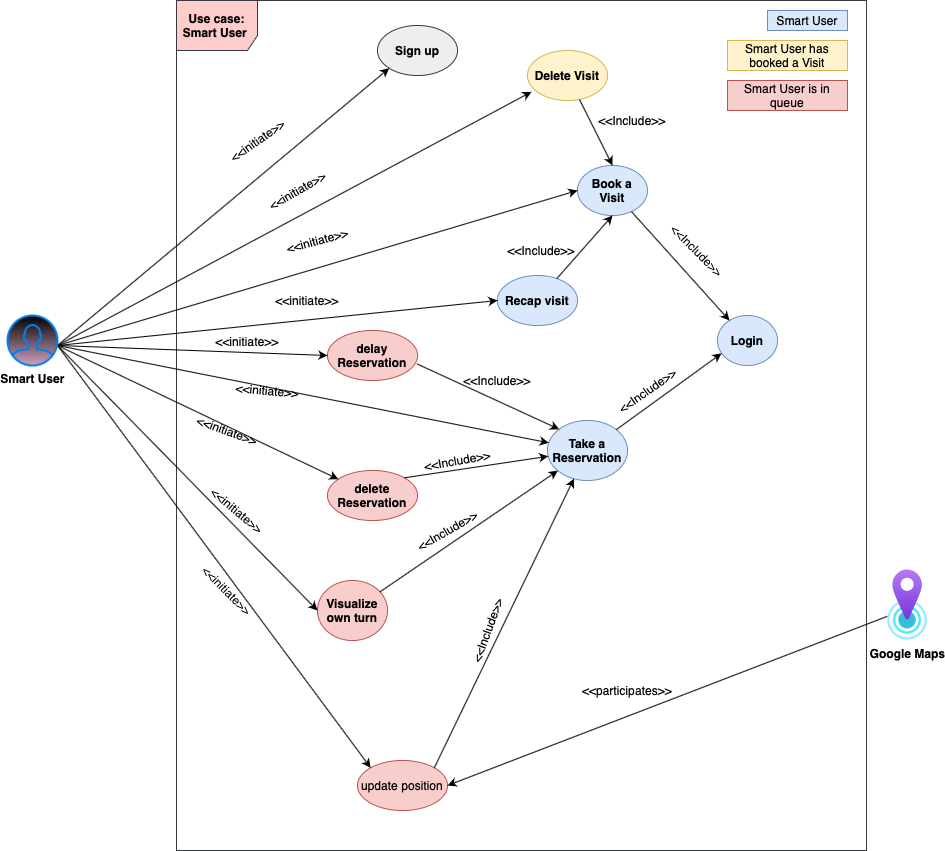
\includegraphics[width=1\textwidth, height=1\textwidth]{diagrams/UseCaseUser.png}
	
\end{figure}

\addvspace{1cm} 
{\normalsize \textbf{Use cases}}
\par \medskip

\begin{tabular}{|p{5cm} | p{7cm} | }
\hline
Name & Login \\
\hline
Actor & User \\
\hline
Entry condition &
\begin{itemize}
\item The user has register
\item The user opened the application
\end{itemize} \\
\hline
Events flow & 
\begin{itemize}
	\item The user open the application
	\item Enters username and password
	\item Click “Login button”
\end{itemize} \\
\hline
Exit condition & User log in \\
\hline 
Exceptions &
\begin{itemize}
	\item User enters wrong username
	\item User enters wrong password
\end{itemize} \\
\hline
\end{tabular}

\par \medskip

\begin{tabular}{|p{5cm} | p{7cm} | }
	\hline
	Name & Sign up \\
	\hline
	Actor & User \\
	\hline
	Entry condition &
	\begin{itemize}
		\item User enters for the first time on the app 
		\item The user hasn’t registered
	\end{itemize} \\
	\hline
	Events flow & 
	\begin{itemize}
		\item The user selects “Create new account” option
		\item The user enters required fields
		\item The user accepts CLup privacy policy
		\item The user clicks “Register” button
	\end{itemize} \\
	\hline
	Exit condition & The users is registered \\
	\hline 
	Exceptions &
	\begin{itemize}
		\item The users has already been registered
		\item The user did not accept CLup privacy policy
		\item The user enters username that has already been used
		\item The user enters prohibited characters
	\end{itemize} \\
	\hline
\end{tabular}

\par \medskip

\begin{tabular}{|p{5cm} | p{7cm} | }
	\hline
	Name & Book a visit \\
	\hline
	Actor & User \\
	\hline
	Entry condition &
	\begin{itemize}
		\item The user has logged in 
	\end{itemize} \\
	\hline
	Events flow & 
	\begin{itemize}
		\item The user click on Home Page
		\item Click on “Book a visit” button
		\item Select the visit date
		\item Select the visit time
		\item Insert shopping size
		\item Click on “Next” button
	\end{itemize} \\
	\hline
	Exit condition & The user book a visit \\
	\hline 
	Exceptions & \\
	\hline
\end{tabular}

\par \medskip

\begin{tabular}{|p{5cm} | p{7cm} | }
	\hline
	Name & Take reservation \\
	\hline
	Actor & User \\
	\hline
	Entry condition &
	\begin{itemize}
		\item The user has logged in 
	\end{itemize} \\
	\hline
	Events flow & 
	\begin{itemize}
		\item The user click on “Home Page” menù
		\item Click on “Reserve a seat” button
		\item Confirm the reservation
	\end{itemize} \\
	\hline
	Exit condition &
	\begin{itemize}	
		\item The user has been queued
		\item The QR code has been associated with user 
	\end{itemize} \\
	\hline 
	Exceptions & The shop is closed \\
	\hline
\end{tabular}

\par \medskip

\begin{tabular}{|p{5cm} | p{7cm} | }
	\hline
	Name & Delete Visit \\
	\hline
	Actor & UserVisiting \\
	\hline
	Entry condition &
	\begin{itemize}
		\item The user has logged in
		\item The user took a visit
	\end{itemize} \\
	\hline
	Events flow & 
	\begin{itemize}
		\item The user clicks on “QR code” menù
		\item The visits and reservation are listed
		\item The user clicks on “Delete” button near the visit
		\item The user confirms the cancellation
	\end{itemize} \\
	\hline
	Exit condition &
	\begin{itemize}	
		\item The system delete user visit
		\item The system make available date and time of user visit
	\end{itemize} \\
	\hline 
	Exceptions & \\
	\hline
\end{tabular}

\par \medskip

\begin{tabular}{|p{5cm} | p{7cm} | }
	\hline
	Name & Delete reservation \\
	\hline
	Actor & UserInQueue \\
	\hline
	Entry condition &
	\begin{itemize}
		\item The user has logged in
		\item The user took a reservation
	\end{itemize} \\
	\hline
	Events flow & 
	\begin{itemize}
		\item The user clicks on “QR code” menù
		\item The visits and reservation are listed
		\item The user clicks on “Delete” button near the reservation
		\item The user confirms the cancellation
	\end{itemize} \\
	\hline
	Exit condition &
	The system delete user reservation \\
	\hline 
	Exceptions & \\
	\hline
\end{tabular}

\par \medskip

\begin{tabular}{|p{5cm} | p{7cm} | }
	\hline
	Name & Delay reservation \\
	\hline
	Actor & UserInQueue \\
	\hline
	Entry condition &
	\begin{itemize}
		\item The user has logged in
		\item The user took a reservation
	\end{itemize} \\
	\hline
	Events flow & 
	\begin{itemize}
		\item The user clicks on “QR code” menù
		\item The visits and reservation are listed
		\item The user clicks on “Delay” button near the reservation
		\item The user confirms the delay
	\end{itemize} \\
	\hline
	Exit condition &
	\begin{itemize}
		\item The user turn will be shift ten places after.
		\item The delay button will be disabled.
	\end{itemize} \\
	\hline 
	Exceptions & 
	\begin{itemize}
		\item The user queue is too small
		\item The user delay function has already been used
	\end{itemize} \\
	\hline
\end{tabular}

\par \medskip

\begin{tabular}{|p{5cm} | p{7cm} | }
	\hline
	Name & Recap visit \\
	\hline
	Actor & User \\
	\hline
	Entry condition &
	The user has logged in \\
	\hline
	Events flow & 
	The user click on “history” menù \\
	\hline
	Exit condition &
	The visits and reservation are listed \\
	\hline 
	Exceptions & \\
	\hline
\end{tabular}

\par \medskip

\begin{tabular}{|p{5cm} | p{7cm} | }
	\hline
	Name & Visualize own turn \\
	\hline
	Actor & UserInQueue \\
	\hline
	Entry condition &
	\begin{itemize}
		\item The user has logged in
		\item The user took a reservation
	\end{itemize} \\
	\hline
	Events flow & 
	The user clicks on “history” menù \\
	\hline
	Exit condition &
	The system show the user turn near the reservation QR code \\
	\hline 
	Exceptions & \\
	\hline
\end{tabular}

\par \medskip

\begin{tabular}{|p{5cm} | p{7cm} | }
	\hline
	Name & Update position  \\
	\hline
	Actor & UserInQueue \\
	\hline
	Entry condition &
	\begin{itemize}
		\item The user has logged in
		\item The user took a reservation
	\end{itemize} \\
	\hline
	Events flow & 
	\begin{itemize}
		\item The user clicks on “QR code” menù
		\item The user clicks on “Update position”
	\end{itemize} \\
	\hline
	Exit condition &
	The system calculate the number of customers in queue after which will send the message  \\
	\hline 
	Exceptions & 
	\begin{itemize}
		\item GPS position too far from supermarket
		\item Invalid GPS position
		\item GPS is inactive
	\end{itemize} \\
	\hline
\end{tabular}

\par \medskip

\begin{tabular}{|p{5cm} | p{7cm} | }
	\hline
	Name & Choice market  \\
	\hline
	Actor & User \\
	\hline
	Entry condition &
	User login for the first time on the app \\
	\hline
	Events flow & 
	\begin{itemize}
		\item Select the supermarket
		\item Click “Next” to confirm
	\end{itemize} \\
	\hline
	Exit condition &
	The system calculate the number of customers in queue after which will send the message  \\
	\hline 
	Exceptions & 
	The user is linked to supermarket \\
	\hline
\end{tabular}

\par \medskip

\subsection{Reception}
\par \medskip
{\large \textbf{Scenarios}}
\par \medskip
{\normalsize \textbf{Scenario 1}}
\par \medskip
 Gustavo, an elderly person, he discovered recently a new time saver and usefull service at the market. \\
 It consists to book a visit at the market by simply calling the number found in an advertisment. \\
 Due to the fact that Gustavo is sick of waiting too much in the queue decide to call this market number to book the visit. \\
 On the other side Marta, a gentle receptionist who works for the market, answers to Gustavo's call; she takes care of the registration of his own data, the credentials and the all visit information (i.e data and range time).\\
  Gustavo will be notified about the appointment with an SMS on his mobilephone in time. \\
  In addition the SMS will provide the schedule for the visit and the code which will be submitted at the entrance.
 
 \par \medskip 
 
 \begin{figure}[h]
 	\caption{Use case RECEPTION}
 	\label{fig:UML}
 	
 	\centering
 	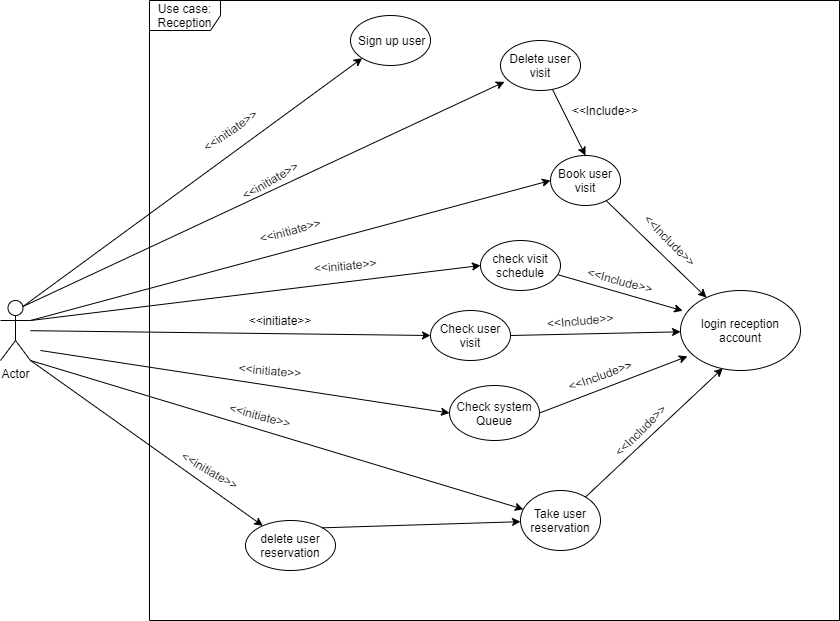
\includegraphics[width=1\textwidth, height=1\textwidth]{diagrams/UseCaseReception.png}
 	
 \end{figure}
 
 
 

\section{Performance Requirements}
\section{Design Constraints}
\subsection{Standards compliance}
\subsection{Hardware limitations}
\subsection{Any other constraint}

\section{Software System Attributes}
\subsection{Reliability}
\subsection{Availabilitys}
\subsection{Security}
\subsection{Maintainability}
\subsection{Portability}
